% !TEX program = lualatex
\documentclass[12pt,ngerman]{scrartcl}

% KOMA-Script Artikel-Praeambel passend zur AVVP-Beamer-Vorlage (Magazin-Look)
% Engine: LuaLaTeX (wegen fontspec und lokaler OTF/TTF)

\usepackage[ngerman]{babel}
\usepackage{fontspec}
\usepackage{xcolor}
\usepackage{graphicx}
\usepackage{csquotes}
\usepackage{microtype}
\usepackage{hyperref}

% Bibliographie wie im Beamer-Projekt
\usepackage[style=authoryear]{biblatex}
\addbibresource{bibtex.bib}

\usepackage{booktabs}
\usepackage{etoolbox}
\usepackage{float}

% Optional: Seitenlayout
\usepackage[a4paper,margin=2.5cm]{geometry}

% Kopf-/Fußzeile (Magazin)
\usepackage[automark,headsepline]{scrlayer-scrpage}
\usepackage{lastpage}

% Kopf-/Fußzeilen-Inhalt
\clearpairofpagestyles
\automark{section}
\ihead{\headmark}

% Rechts oben: Titel (Kurztitel, falls via \title[Kurztitel]{...} gesetzt)
\makeatletter
\newcommand{\AVVPHeaderTitle}{%
  \ifcsname shorttitle\endcsname
    \ifx\shorttitle\@empty
      \@title
    \else
      \shorttitle
    \fi
  \else
    \@title
  \fi
}
\makeatother
\ohead{\AVVPHeaderTitle}

\cfoot{Seite\ \pagemark\ von\ \pageref{LastPage}}
\pagestyle{scrheadings}

% Farben (aus dem Beamer-Theme uebernommen)
\definecolor{AVVPBg}{RGB}{5,23,41}
\definecolor{AVVPBlue}{RGB}{46,108,198}
\definecolor{AVVPSpark}{RGB}{235,156,70}
\definecolor{AVVPGrey}{RGB}{90,98,110}

% Schriften (lokal aus dem Projekt)
\setmainfont[
  Path = fonts/exo-2/,
  Extension = .otf,
  UprightFont = *-Regular,
  ItalicFont  = *-Italic,
  BoldFont    = *-Bold,
  BoldItalicFont = *-BoldItalic,
  Ligatures = TeX
]{Exo2}

\setsansfont[
  Path = fonts/exo-2/,
  Extension = .otf,
  UprightFont = *-Regular,
  ItalicFont  = *-Italic,
  BoldFont    = *-Bold,
  BoldItalicFont = *-BoldItalic,
  Ligatures = TeX
]{Exo2}

\newfontfamily\AVVPTitleFont[
  Path = fonts/share_techmono/,
  Extension = .otf,
  UprightFont = Share-TechMono,
  Ligatures = {TeX,NoCommon}
]{Share Tech Mono}

% Ueberschriften in CI-Farbe
\addtokomafont{disposition}{\color{AVVPBlue}\AVVPTitleFont}

% AVVP Link-Farbe
\hypersetup{colorlinks=true,linkcolor=AVVPBlue,urlcolor=AVVPBlue,citecolor=AVVPBlue}

% Default fuer \includegraphics: volle Textbreite, Seitenverhaeltnis behalten
\setkeys{Gin}{width=\linewidth,keepaspectratio}



% --- Magazin-Look: weniger Weißraum + ruhigere Captions ---
\setlength{\textfloatsep}{6pt plus 2pt minus 2pt}
\setlength{\intextsep}{6pt plus 2pt minus 2pt}
\setlength{\floatsep}{6pt plus 2pt minus 2pt}
\setlength{\abovecaptionskip}{3pt}
\setlength{\belowcaptionskip}{0pt}

% Abbildungen/Tabellen im Artikel möglichst "hier" setzen
\floatplacement{figure}{H}
\floatplacement{table}{H}

% Linksbuendig in figure/table, auch wenn im Dokument \centering steht
\AtBeginEnvironment{figure}{\let\centering\raggedright}
\AtBeginEnvironment{table}{\let\centering\raggedright}

% Captions kleiner, grauer und linksbuendig
\makeatletter
\long\def\@makecaption#1#2{%
  \vskip\abovecaptionskip
  {\footnotesize\color{AVVPGrey}#1: #2\par}%
  \vskip\belowcaptionskip
}
\makeatother

% ------------------------------------------------------------
% Bildnachweis (Artikel): kompatible Kurzform wie im Beamer (cite-key)
%   Nutzung: \AVVPCreditInline{cite-key}
% ------------------------------------------------------------
\makeatletter
\newcommand{\AVVPCreditInline}[1]{%
  \begingroup
    \@ifpackageloaded{biblatex}{\nocite{#1}}{}%
    \;\textnormal{([#1])}%
  \endgroup
}
\makeatother

% ------------------------------------------------------------
% VIDEO HELPERS (wie in der Beamer-Präambel; Artikel-Implementierung)
%   Ziel: gleiche Makro-Namen/Signaturen, aber Magazin-taugliche Ausgabe.
% ------------------------------------------------------------

% Poster-Image (skalieren ohne Verzerrung, Hoehe begrenzen)
\newcommand{\AVVPVideoPoster}[2][]{%
  \includegraphics[
    width=0.5\linewidth,
    height=0.35\textheight,
    keepaspectratio,
    #1%
  ]{#2}%
}

% Minimaler File-URI Builder (ersetzt Leerzeichen durch %20)
\makeatletter
\ExplSyntaxOn
\tl_new:N \g_avvp_file_uri_tl
\cs_new_protected:Npn \avvp_build_file_uri:n #1
  {
    \tl_set:Nn \l_tmpa_tl {#1}
    \tl_replace_all:Nnn \l_tmpa_tl {\c_space_tl} {\c_percent_str 20}
    \tl_gset:Nx \g_avvp_file_uri_tl { run:\tl_use:N \l_tmpa_tl }
  }
\newcommand{\AVVPBuildFileURI}[1]{%
  \begingroup
    \avvp_build_file_uri:n {#1}%
    \xdef\AVVPFileURI{\tl_use:N \g_avvp_file_uri_tl}%
  \endgroup
}
\ExplSyntaxOff
\makeatother

% Label wie in Beamer: nur "ordner/datei" (fallback: kompletter String)
\makeatletter
\ExplSyntaxOn
\cs_new_protected:Npn \avvp_video_local_label:n #1
  {
    \seq_set_split:Nnn \l_tmpa_seq {/} {#1}
    \int_compare:nNnTF {\seq_count:N \l_tmpa_seq} > {1}
      {
        \tl_set:Nx \l_tmpb_tl {\seq_item:Nn \l_tmpa_seq {-2}}
        \tl_set:Nx \l_tmpc_tl {\seq_item:Nn \l_tmpa_seq {-1}}
        \texttt{\nolinkurl{\tl_use:N \l_tmpb_tl/\tl_use:N \l_tmpc_tl}}
      }
      {\texttt{\nolinkurl{#1}}}
  }
\newcommand{\AVVPVideoLocalLabel}[1]{\avvp_video_local_label:n {#1}}
\ExplSyntaxOff
\makeatother

% Clickable poster -> URL
\newcommand{\AVVPVideoURL}[3][]{%
  \begin{center}%
    \href{#2}{\AVVPVideoPoster[#1]{#3}}%
  \end{center}%
}

% Clickable poster -> lokale Datei
\newcommand{\AVVPVideoLocal}[3][]{%
  \begin{center}%
    \AVVPBuildFileURI{#2}% setzt \AVVPFileURI
    \href{\AVVPFileURI}{\AVVPVideoPoster[#1]{#3}}\\[0.4ex]%
    {\scriptsize\href{\AVVPFileURI}{\AVVPVideoLocalLabel{#2}}}%
  \end{center}%
}

% ------------------------------------------------------------
% Quellenverzeichnis wie im Beamer: cite-key [..] am Anfang jeder Zeile
% ------------------------------------------------------------
\makeatletter
\AtBeginDocument{%
  \@ifpackageloaded{biblatex}{%
    \DeclareFieldFormat{entrykey}{[#1]}%
    \renewbibmacro*{begentry}{\printfield{entrykey}\addspace}%
  }{}%
}
\makeatother

% Bildpfade wie in der Beamer-Vorlage (Aufruf aus AVVP_Beamer/)
\graphicspath{{./}{pics/}{media/}}

% ------------------------------------------------------------
% AVVP Titel-Assets (Benennung analog zur Beamer-Praeambel)
% ------------------------------------------------------------
\def\AVVPTitleLogoDarkFile{pics/avvp_2019_logo_wortmarke_neg.png}
\def\AVVPTitleLogoLightFile{pics/avvp_2019_logo_wortmarke_pos_gross.png}
\def\AVVPTitleSloganText{Faszination. Astronomie. Erleben.}

% Modus-Flag analog zum Beamer-Theme
\newif\ifAVVPIsLightMode
% Artikel hat weissen Hintergrund -> default Light
\AVVPIsLightModetrue

\newcommand{\AVVPDarkMode}{\global\AVVPIsLightModefalse}
\newcommand{\AVVPLightMode}{\global\AVVPIsLightModetrue}

\newcommand{\AVVPTitleLogoAuto}{%
  \ifAVVPIsLightMode
    \includegraphics[width=0.30\textwidth]{\AVVPTitleLogoLightFile}%
  \else
    \includegraphics[width=0.30\textwidth]{\AVVPTitleLogoDarkFile}%
  \fi
}

\newcommand{\AVVPTitleSloganColor}{%
  \ifAVVPIsLightMode
    \color{AVVPBg}% dark text on light background
  \else
    \color{white}% light text on dark background
  \fi
}

% Titelseite fuer KOMA-Artikel (Logo + Drei-Zeiler)
\makeatletter
\newcommand{\AVVPMakeTitlePage}{%
  \begin{titlepage}
    \centering

    {\AVVPTitleFont\color{AVVPBlue}\LARGE\@title\par}

    \ifx\@subtitle\@empty\else
      \vspace{0.8em}
      {\AVVPTitleFont\color{AVVPSpark}\large\@subtitle\par}
    \fi

    \vspace{1.2em}
    {\color{AVVPBlue}\begingroup\let\and\\\@author\par\endgroup}

    \vspace{0.6em}
    {\color{AVVPBlue}\@date\par}

    \vfill

    \AVVPTitleLogoAuto\par

    \vspace{0.8em}
    {\AVVPTitleFont\AVVPTitleSloganColor\normalsize\AVVPTitleSloganText\par}

  \end{titlepage}
}
\makeatother

\title{Hauptthema bzw. Titel\\Titel 2. Zeile}
\subtitle{Untertitel, wenn vorhanden}
\author{1.~Author \and 2.~Author}
\date{Vereinsabend, 04.02.2026}

\begin{document}

\AVVPMakeTitlePage
\clearpage
\bigskip

\noindent\textbf{Hinweis (Workflow):} Die Beamer-Präsentation ist die inhaltliche Referenz. Dieser Artikel ist eine abgeleitete Darstellung derselben Inhalte und muss bei Änderungen in der Präsentation entsprechend aktualisiert werden.

\tableofcontents

\section{Motivation}

\subsection{Struktur}

\subsubsection*{Strukturierte Vorträge}

Einen Vortrag zu strukturieren ist nicht immer einfach. Hier ein paar Regeln, die für diese Lösungsvorlage gelten.

\begin{itemize}
\item Konferenzteilnehmer wissen oft wenig von der Materie des Vortrags. Deshalb: vereinfachen!
\item In 20 Minuten ist es schon schwer genug, die Hauptbotschaft zu vermitteln. Deshalb sollten Details ausgelassen werden, selbst wenn dies zu Ungenauigkeiten oder Halbwahrheiten führt.
\item Falls man Details weglässt, die eigentlich wichtig sind, so bitte auf der Tonspur. Alle werden damit glücklich sein.
\end{itemize}

\subsubsection*{Strukturierte Vorträge (2)}

Inhalte sollten in Blöcke gegliedert sein und damit zu einem klar umrissenen Ziel führen.

\begin{itemize}
\item Es sollte genau zwei oder drei Abschnitte geben (neben der \% Zusammenfassung).
\item {*}Höchstens{*} drei Unterabschnitte pro Abschnitt.
\item Pro Rahmen sollte man zwischen 30s und 2min reden. Es sollte also 15 bis 30 Rahmen geben.
\end{itemize}

\subsection{LaTeX und LyX}

\subsubsection*{Warum LaTeX Beamer für Präsentationen?}

\begin{figure}
  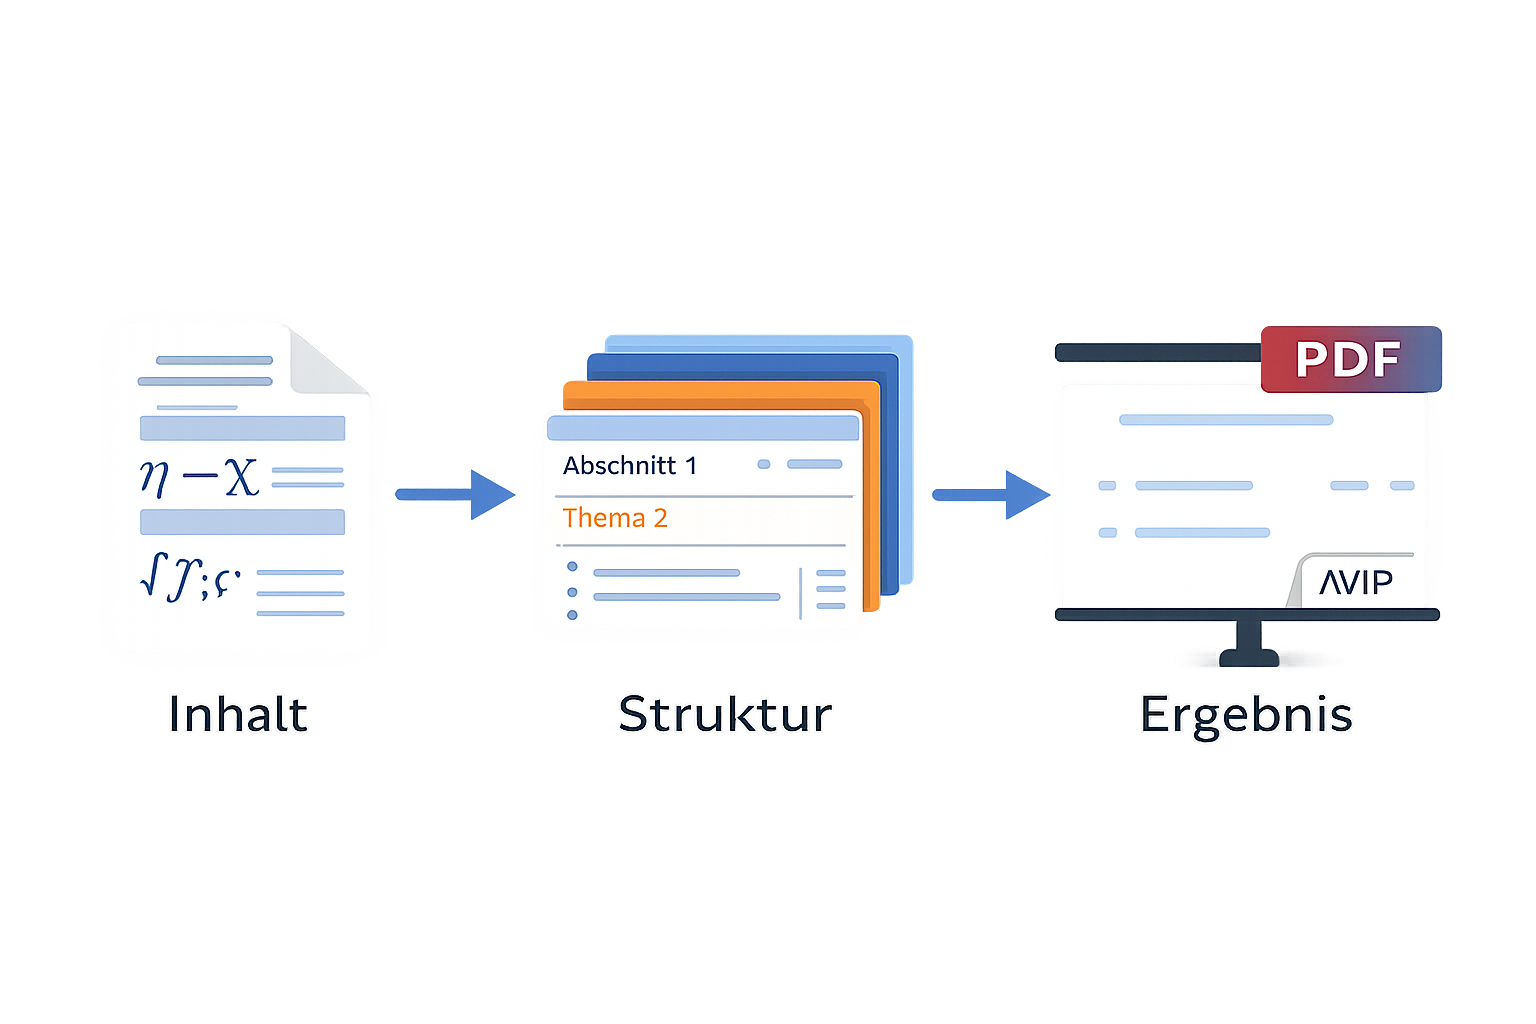
\includegraphics{latex_prinzip_nur_bild_trans}
  \caption{Prinzipdarstellung}
\end{figure}

\begin{itemize}
\item Klare Trennung von Inhalt und Layout
\item Einheitliches Erscheinungsbild über alle Folien
\item Automatische Struktur durch Abschnitte, Unterabschnitte und Agenda
\item Sehr gut geeignet für Formeln, Abbildungen und Referenzen
\item Stabil und skalierbar auch bei großen Präsentationen
\item Textbasierte Quellen ermöglichen Versionierung und langfristige Reproduzierbarkeit
\end{itemize}

\subsubsection*{Warum LyX in Kombination mit Beamer?}

\begin{figure}[h]
  \centering
  
\includegraphics[width=0.15\linewidth]{latex-logo-png_seeklogo-82426_weiss.png}
  \hspace{2em}
  
\includegraphics[width=0.15\linewidth]{org.lyx.LyX.png}
  \caption{LaTeX + LyX}
\end{figure}

\begin{figure}
  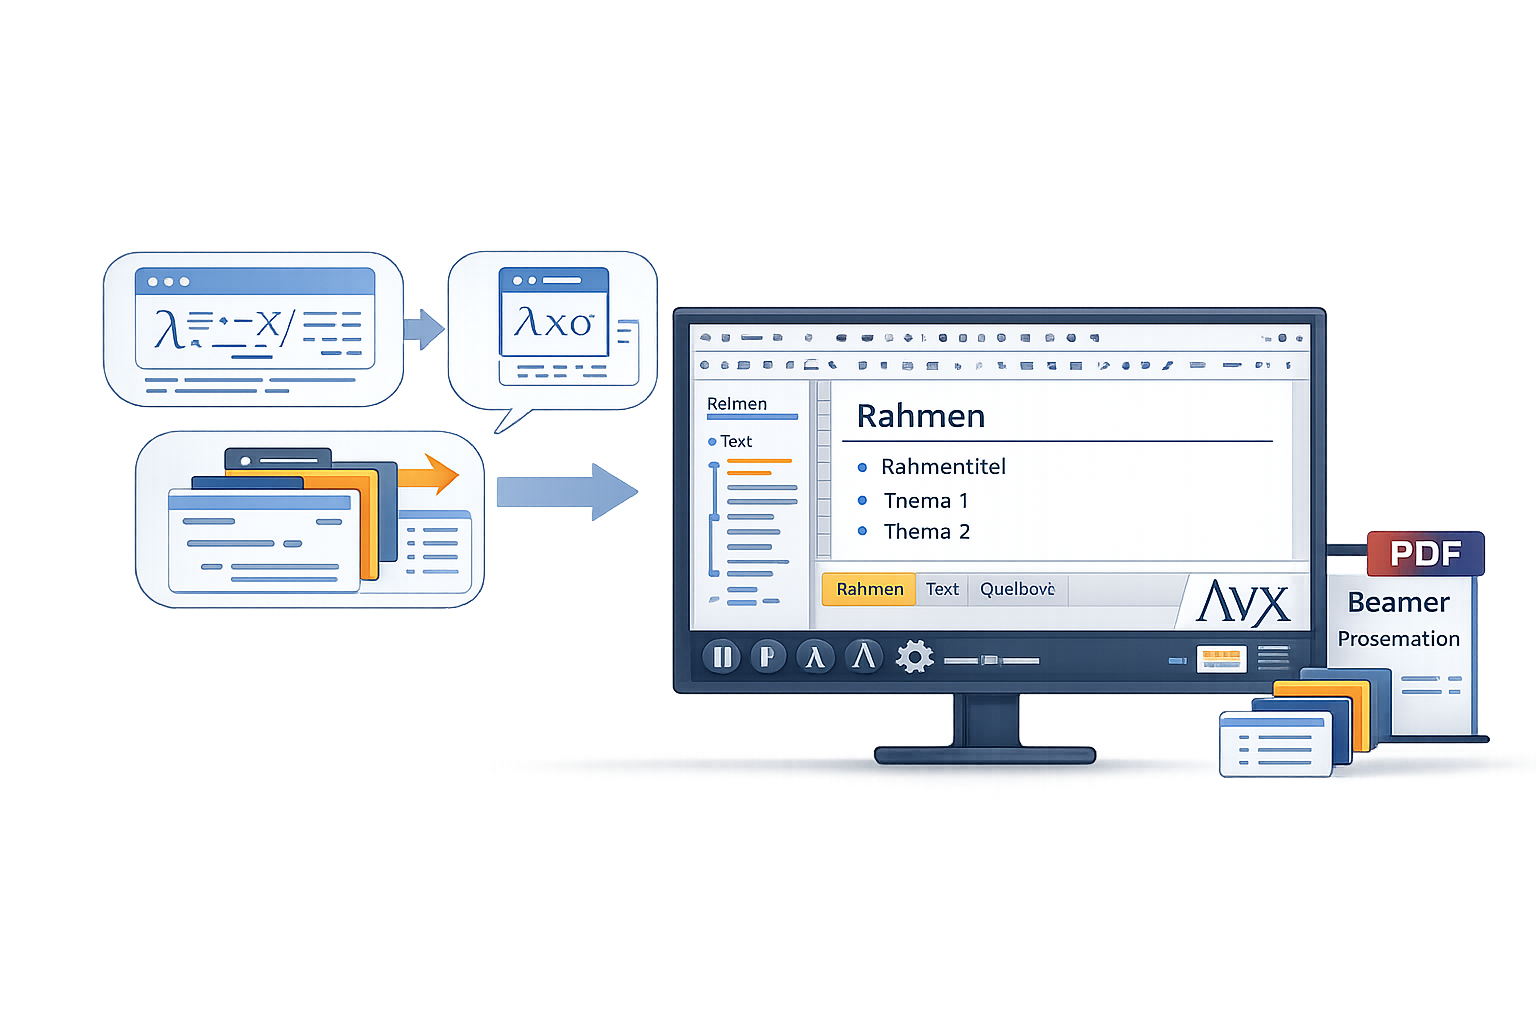
\includegraphics{lyx_prinzip_bildfuellend_breiter_trans}
  \caption{LyX-Prinzip}
\end{figure}

\begin{itemize}
\item Grafische Oberfläche für LaTeX ohne manuelles Tippen von Code
\item Strikte Strukturierung: Dokument, Abschnitte und Rahmen
\item Saubere Trennung zwischen Inhaltserstellung und Design
\item Ideal für kollaboratives Arbeiten und spätere Pflege
\item Volle LaTeX-Leistung bleibt jederzeit verfügbar
\end{itemize}

\section{Text}

\subsection{Aufzählungen}

\subsubsection*{Itemize und Statements}

\textit{Untertitel sind optional.}

Folgende Itemize-Regeln sind ganz nützlich:
\begin{itemize}
\item Viel Itemize benutzen.
\item Sehr kurze Sätze oder Satzglieder verwenden.
\item Diese Overlays werden mit dem Pause Stil erzeugt.
\end{itemize}

Und natürlich Aufzählungen:
\begin{enumerate}
\item Now lets numerate
\item and two
\item and three
\end{enumerate}

\subsubsection*{Konzentration auf einzelne Punkte}

\begin{itemize}
\item Man kann auch Overlay-Spezifikationen benutzen, um Overlays zu erzeugen.
\item Hiermit können, Punkte in beliebiger Reihenfolge präsentiert werden
\item Dies wird als zweites gezeigt.
\end{itemize}

\subsection{Spezielle Umgebungen}

\subsubsection*{Satz / Folgerung}

\paragraph{Theorem.} Auf dem ersten Overlay.

\paragraph{Corollary.} Auf dem zweiten Overlay.

\subsubsection*{Blocks}

\paragraph{Normaler Block.}
\begin{itemize}
\item Wird auf allen Overlays angezeigt.
\end{itemize}

\paragraph{Beispielblock.}
Ein Beispielblocktitel

\begin{itemize}
\item $e^{i\pi}=-1$.
\item $e^{i\pi/2}=i$.
\end{itemize}

\subsubsection*{Definitionen}

\paragraph{Definition.} Hier steht eine Definition.

\paragraph{Beispiel.} Und hier ein Beispiel.

\paragraph{Beweis.} Und hier der Beweis.

\subsubsection*{Quellcode}

Dies ist ein Programm-Listing in \TeX innerhalb von LyX.

\begin{verbatim}
\begin{itemize}
\item $e^{i\pi}=-1$.
\item $e^{i\pi/2}=i$.
\end{itemize}
\end{verbatim}

\section{Tabellen}

\subsection{Alleinstehend}

\subsubsection*{Tabelle mit Überschrift}

\begin{table}[h]
\centering
\caption{Tabelle mit Überschrift}
\begin{tabular}{|c|c|c|c|}
\hline
Lorem & ipsum & dolor & amet \\
\hline
\hline
orem ipsum &  &  & orem iplor s \\
\hline
 & orem dolor s &  \\
\hline
 &  & orem dolor s &  \\
\hline
\end{tabular}
\end{table}

\section{Medien}

\subsection{Einzelnes Bild}

\begin{figure}
  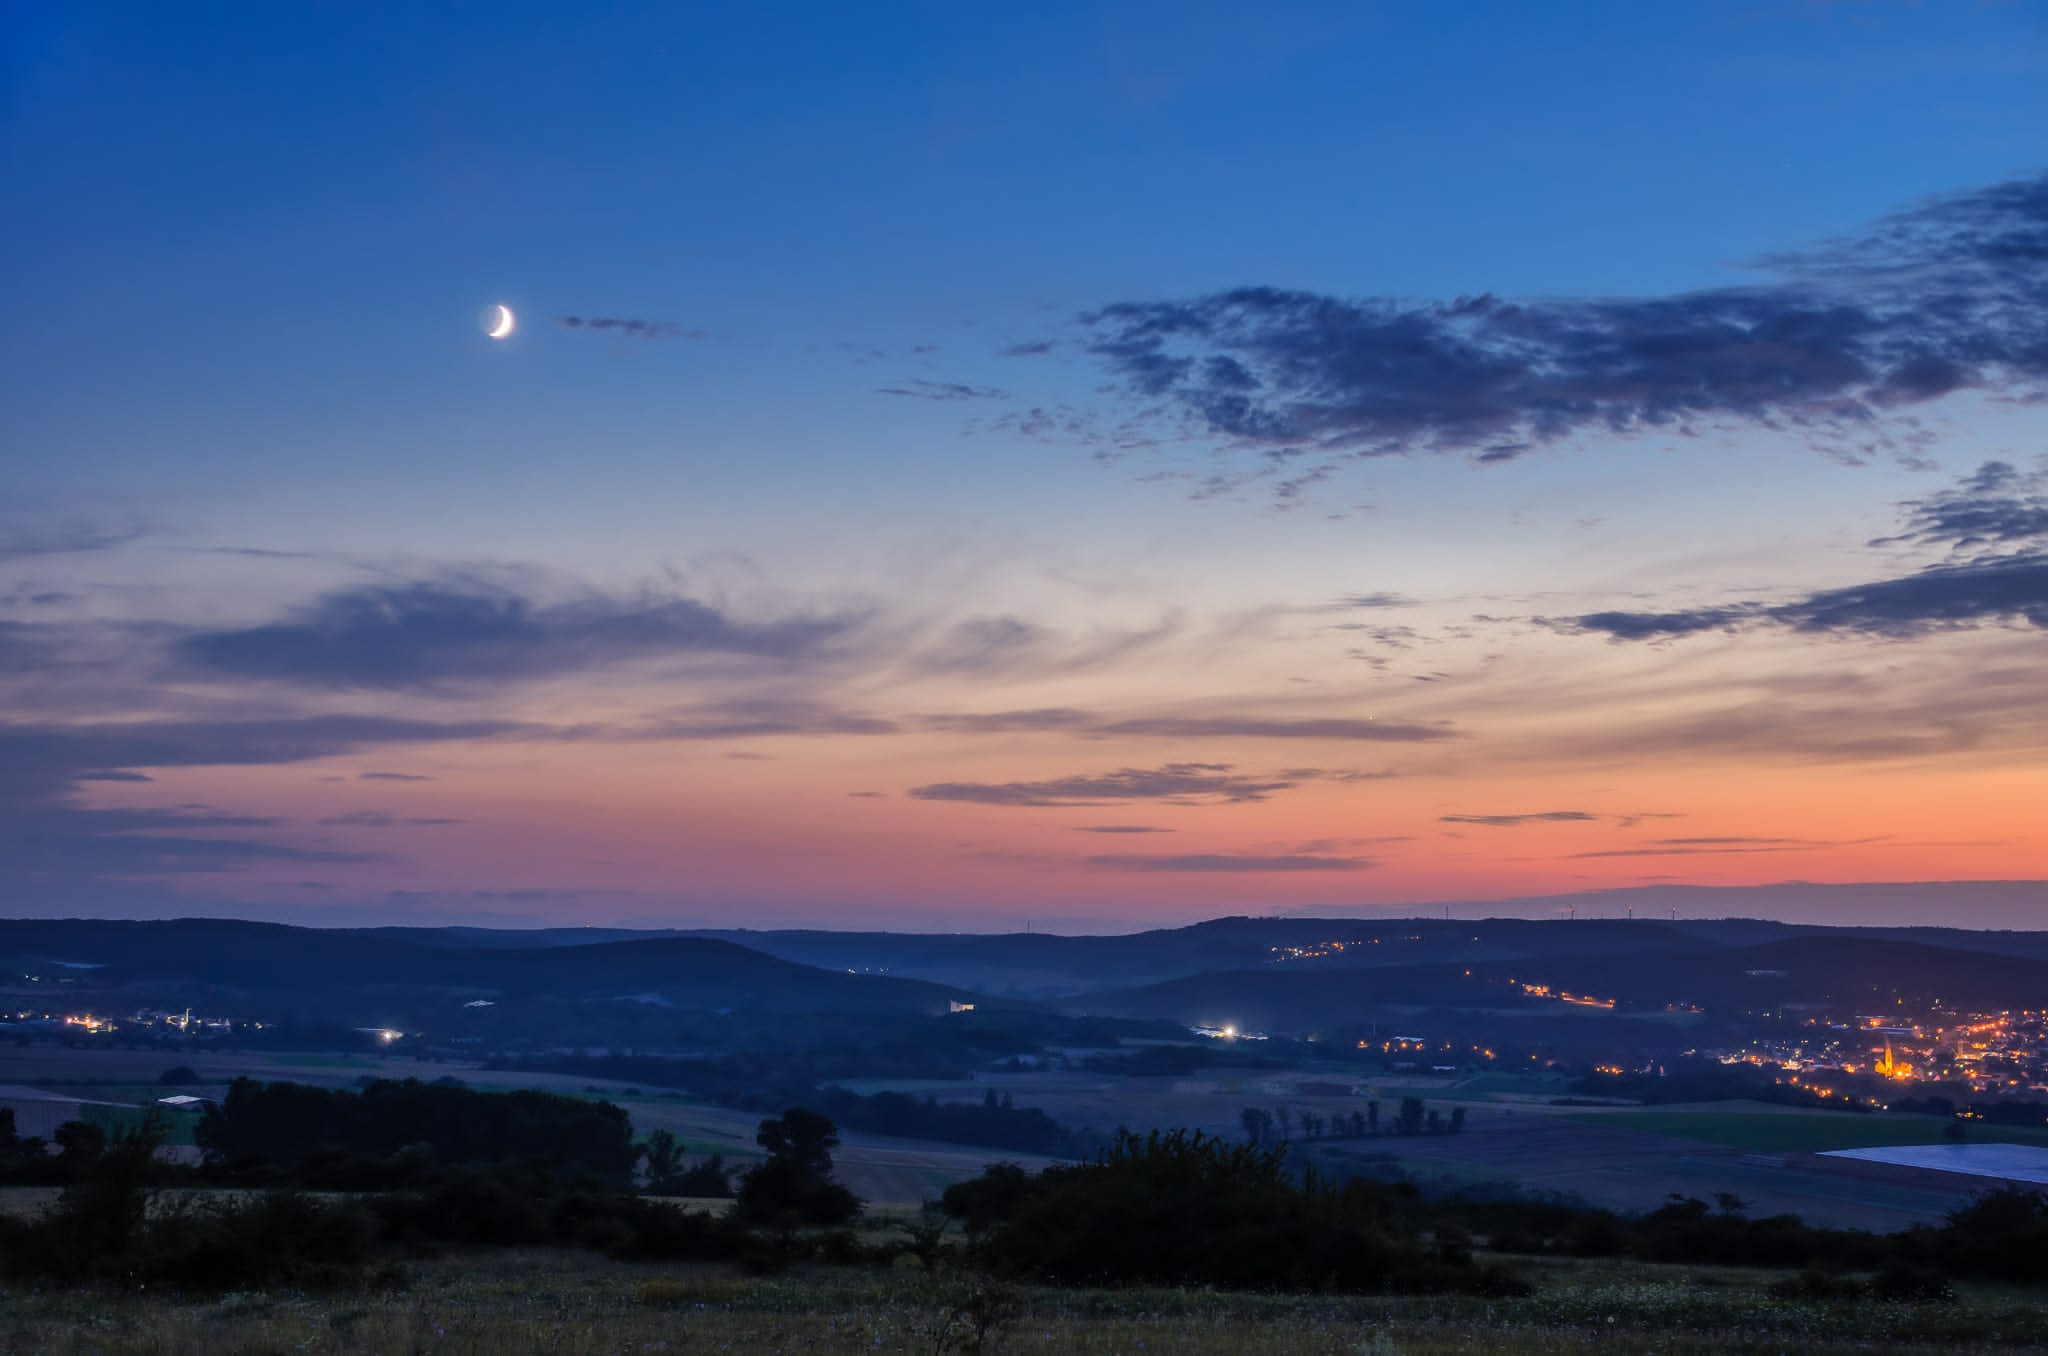
\includegraphics{EVZL1977.JPG}
  \caption{Bild\AVVPCreditInline{hajnal-haslach-2025}}
\end{figure}

\subsection{Bild mit Text}

\subsubsection*{Bild mit Überschrift}

Die Rahmenoption \texttt{<{*}>} führt dazu, dass alles in einem \glqq Rutsch\grqq{} angezeigt wird. Keine Klicks.

\begin{figure}
  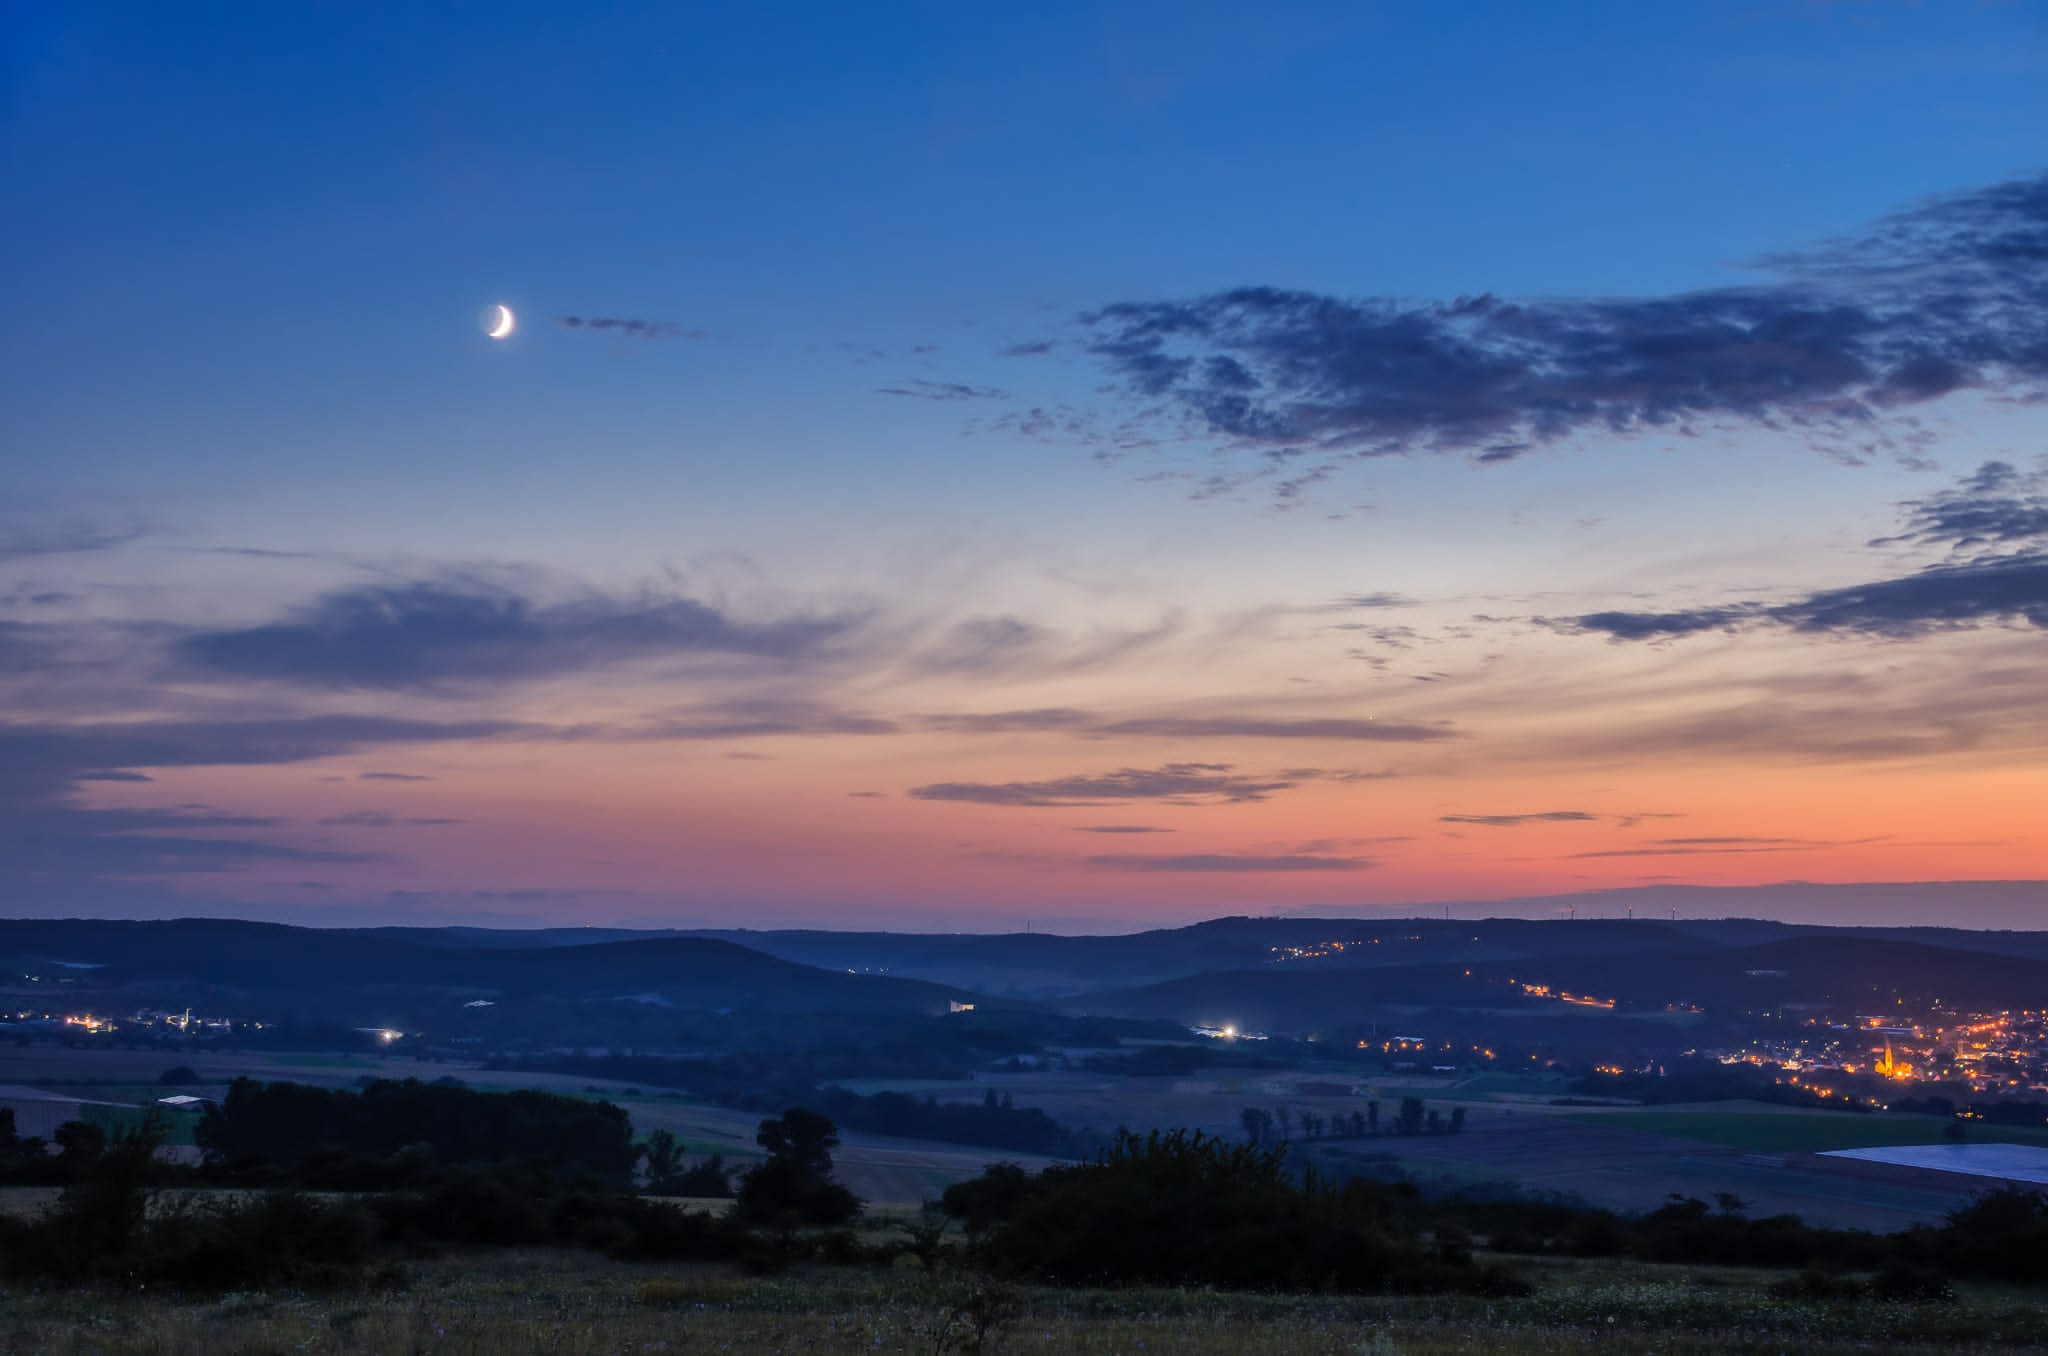
\includegraphics{EVZL1977.JPG}
  \caption{Bild\AVVPCreditInline{hajnal-haslach-2025}}
\end{figure}

\subsubsection*{Bild ohne Überschrift (plain)}

\begin{itemize}
\item Bild ohne Überschrift - voller Fokus aufs Bild
\item daher auch Frame-Option \texttt{plain}
\item Einzelnes Bild mit Quellennachweis
\end{itemize}

\begin{figure}
  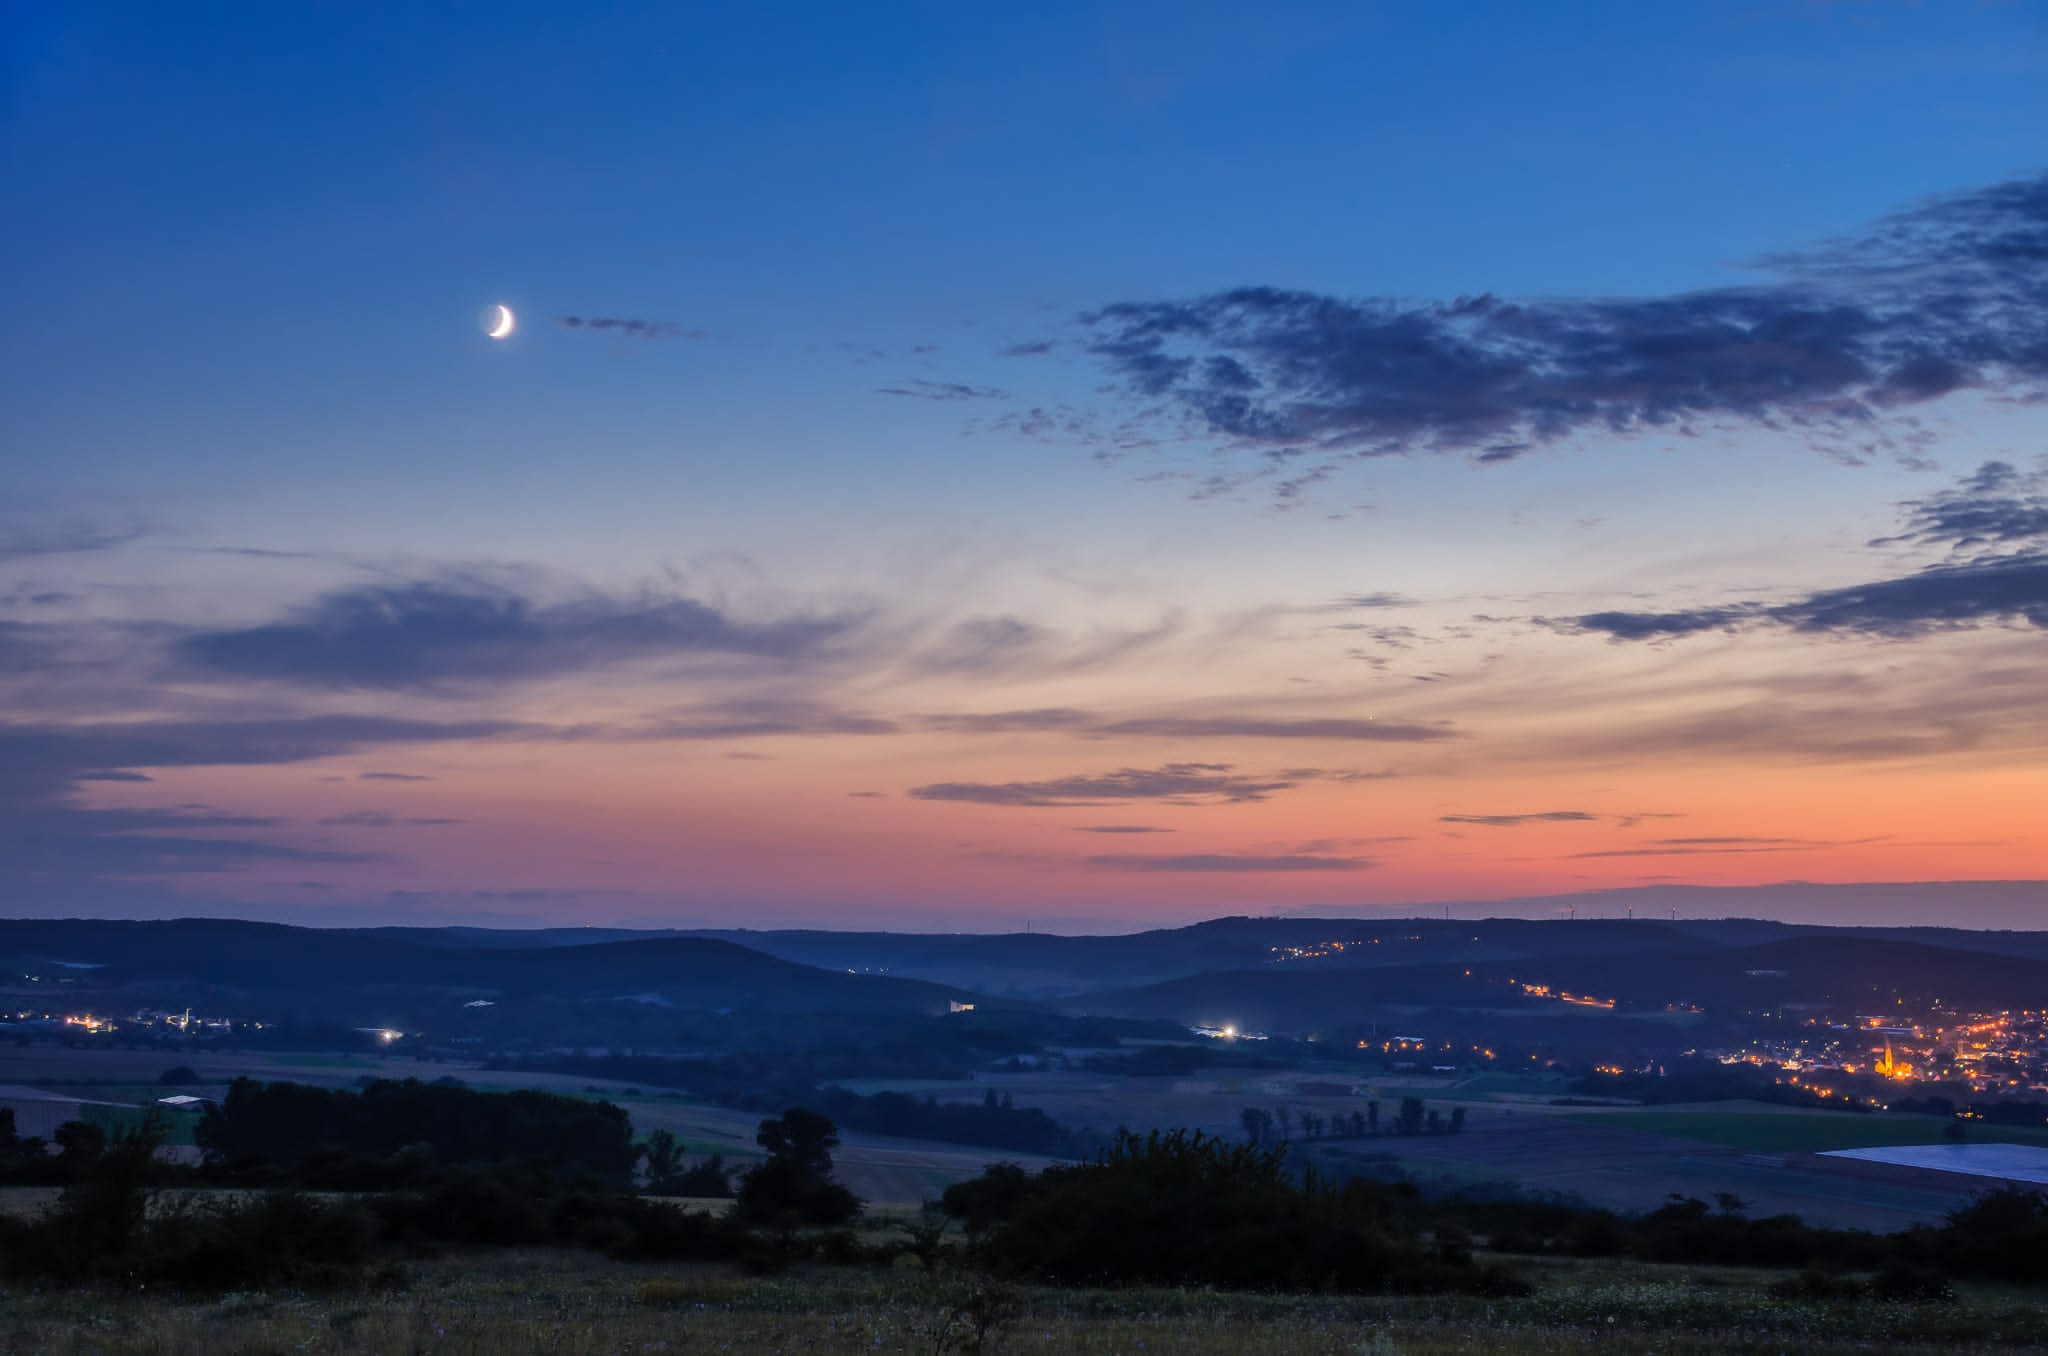
\includegraphics{EVZL1977.JPG}
  \caption{Bild\AVVPCreditInline{hajnal-haslach-2025}}
\end{figure}

\subsubsection*{Bild im Hintergrund}

\begin{itemize}
\item Bild im Hintergrund und ohne Überschrift
\item Einzelnes Bild mit Quellennachweis
\item Platz für Bulletpoints
\end{itemize}

\subsubsection*{Gif}

\begin{itemize}
\item Ein Gif-Bild oder viele andere Dateien können im PDF-Viewer nicht angezeigt werden.
\item Es muss daher als lokale Datei abgelegt und ein separates Vorschaubild verwendet werden.
\item Öffnen funktioniert in vielen PDF-Viewern nicht; ggf. Link kopieren.
\end{itemize}

\begin{figure}
  \AVVPVideoLocal{media/GIF-Bild-4B7D-B0F3-E5-0.gif}{GIF-Bild-4B7D-B0F3-E5-0.png}
  \caption{Gif-Vorschau}
\end{figure}

\subsection{Videos}

\subsubsection*{Video per Youtube-Link}

\noindent\url{https://www.youtube.com/watch?v=eTOM_303DC8}

\begin{figure}
  \AVVPVideoURL{https://www.youtube.com/watch?v=eTOM_303DC8}{YT-TMS-Astro-2-unboxing-deep-inspection.png}
  \caption{YouTube-Video\AVVPCreditInline{yt-heyapos-tms-astro-2-2025}}
\end{figure}

\subsubsection*{Google Drive Link}

\noindent\url{https://drive.google.com/file/d/1erqrKUuNd9FtK19vyPEFOcITf_D7LrFN/view?usp=sharing}

\begin{figure}
  \AVVPVideoURL{https://drive.google.com/file/d/1erqrKUuNd9FtK19vyPEFOcITf_D7LrFN/view?usp=sharing}{AVVP_Universe_on_tour_2024_gdrive.png}
  \caption{Google Drive\AVVPCreditInline{avvp-eV-club-universe-on-tour-2024}}
\end{figure}

\subsubsection*{Lokale Videodatei}

\begin{figure}
  \AVVPVideoLocal{media/Youtube Intro HeyApos longer.mp4}{Youtube_hey_apos_video_jingle_longer.png}
  \caption{Video-Poster\AVVPCreditInline{yt-heyapos-intro-2025}}
\end{figure}

\section*{Zusammenfassung}

\begin{enumerate}
\item Die erste Hauptbotschaft des Vortrags in ein bis zwei Zeilen.
\item Die zweite Hauptbotschaft des Vortrags in ein bis zwei Zeilen.
\item Eventuell noch eine dritte Botschaft, aber nicht noch mehr.
\end{enumerate}

\begin{itemize}
\item Ausblick
  \begin{itemize}
  \item Etwas, was wir noch nicht lösen konnten.
  \item Nochwas, das wir noch nicht lösen konnten.
  \item Uns noch eins
  \end{itemize}
\end{itemize}

\appendix
\section*{Anhang}

\subsection*{Weiterführende Literatur}

\printbibliography[title={Quellenverzeichnis}]

\end{document}